\chapter{预渲染框架设计思路}

预渲染框架整体分为两部分:经过修改的 PreloadLinearLayoutManager 和派发卡片可见性事件的 ViewHolderVisibilityDispatcher。前者主要是替代原有的 LinearLayoutManager,用于实现多种模式的预渲染。同时也对一些由于预加载导致的异常情况进行了修正;后者是由于原来的数据绑定无法再被用于确定卡片是否对用户可见,从而引入的新的生命周期分发器。业务方可以通过注册卡片的可见性来进行监听,并将原来依赖于数据绑定的行为(如曝光埋点)迁移至新的回调方法中。下面对于两个组件的具体结构进行说明。

\section{实现预渲染逻辑}

LinearLayoutManager 允许提供额外的布局空间,来处理布局过程中对对超出屏幕的部分进行布局的特殊要求。方式是通过重写 getExtraLayoutSpace() 方法或者 calculateExtraLayoutSpace() 方法。其中前者只能向一个方向进行布局,后者可以在两个方向进行布局。但是,如果采用后者的话,没有引入 AndroidX 1.1.0 的项目无法使用。所以使用兼容性更强的 getExtraLayoutSpace()。

在该方法中,可以返回一个整型变量来标识需要额外布局多长的布局空间。因为我们需要额外布局一张卡片(也就是下一个视频的信息),所以返回的距离应该为一张卡片的高度。通常情况下,卡片的宽高信息可以直接通过 LayoutManager 获取到,高度通常为屏幕的高度。

通过这个简单的操作,就已经能够实现预渲染的核心逻辑,并且经过验证已经可以提前绑定下一张卡片的数据。然而,通过验证目前的生命周期,我们可以发现,这样的行为其实和没有预渲染并没有什么不同。我们通过一个例子来进行说明:当前卡片为卡片1,在这个情况下,卡片2会因为额外布局空间也被绑定并创建 View 的实例。这样确实能够达到预渲染的效果;然而,如果用户开始向下滑动,在滑动的一瞬间就会因为额外布局空间,将卡片3也提前创建并绑定。在这种情况下,依然会在滚动的过程中进行数据绑定,只不过从原来的提前一张卡片变成了提前两张卡片,耗时逻辑依然会影响主线程的性能。所以,我们需要对额外布局空间进行限制,只有在应用程序相对空闲的时刻才允许额外的布局空间。反映到业务方就是,选择一个更好的时机去进行预渲染。

为此,设计了若干种预渲染模式,来应对不同业务的需求。主要分为:

\begin{itemize}
    \item 没有预渲染(默认情况);
    \item 永远预渲染;
    \item 滚动停止时触发预渲染;
    \item 通过外界触发预渲染。
\end{itemize}

其中,通过外界触发预渲染的模式还可以分为有超时补发机制和没有超时补发机制。在有超时补发机制的版本中,当滚动停止时,如果外界没有立刻进行预渲染调用,那么就会提交一个默认为5秒的任务。当到达规定时间时外界依然没有触发预渲染,那么就会补发一次预渲染来应对一些异常情况。想要让 LayoutManager 在这些不同的预渲染模式中自如切换是需要经过缜密的设计和严谨的测试的,接下来介绍为了迎合不同的模式进行的工作。

RecyclerView 会分发滚动状态的变化。RecyclerView 的滚动状态一共有三种:

\begin{itemize}
    \item SCROLL\_STATE\_IDLE:静止状态;
    \item SCROLL\_STATE\_DRAGGING:滚动状态,不过是用户将手放在屏幕上时;
    \item SCROLL\_STATE\_SETTLING:滚动状态,用户松手后,还会滑动一段距离直到停止。这段过程的状态就是 SETTLING。
\end{itemize}

当 RecyclerView 处理用户的触摸事件时,会根据具体情况设置滚动状态的标记位,并通过回调方法派发滚动状态改变的生命周期。因此我们可以在回调中监听到新的滚动状态,并针对具体的预渲染模式进行预渲染的派发。当预渲染模式为滚动停止触发预渲染时,如果检测到已经滚动停止,那么应该移除已经存在的预渲染任务,并手动提交一次新的预渲染任务;当预渲染模式为带有超时补发机制的外界触发预渲染时,如果检测到滚动停止,那么会在规定的超时时间后手动提交一次新的预渲染任务。

加入了这些回调逻辑之后,需要对 LayoutManager 的 getExtraLayoutSpace() 做进一步特殊处理。由于我们不会永远预渲染,返回的额外布局空间就不会是一个定值。我们需要针对不同的预渲染模式,根据具体的情况进行判断。如果是滚动停止触发预渲染的模式,只有在当前 RecyclerView 不为滚动状态时才返回额外的布局空间,否则返回默认值0;如果是外界触发的预渲染,那么绝大多数情况都应该返回默认值,只有外界触发预渲染的那一刻才返回额外的布局空间用于预渲染。

以上的逻辑可以满足大部分预渲染的场景。但是,由于没有经过完善的测试,这样的逻辑依然隐藏了一些缺陷。这里主要介绍一下针对预渲染框架进行的额外工作;在下一章会介绍测试环节中出现的缺陷及其解决思路和过程。

主要的额外工作都在外界触发预渲染上,因为外界触发预渲染的时机不能保证。准确地说,无法确保外界触发预渲染时,RecyclerView 一定处于滚动停止状态。因此需要引入不同于超时补发预渲染机制的另一种补发预渲染的时机:当外界触发预渲染时,如果 RecyclerView 还不处于滚动停止状态,那么需要等到滚动停止时进行补发。这样做的一个主要原因是,在视频场景的 Feed 流中,通常外界触发预渲染的时机是视频起播的时机。但是视频起播通常和滚动停止互为异步行为。这样做的目的是为了优化起播的速度,用户滑动到当前视频,在卡片停稳之前就能做一些初始化的工作,从而让用户感觉视频的播放更加流畅。而如果视频起播时卡片仍然在滑动(性能越强的手机越容易出现这种情况),那么就违背了让预渲染任务避开卡片滑动事件的初心。因此需要做这样一个补发机制,来让外界触发的预渲染一定是在卡片静止时进行的。为此设置了如下标记位来记录外界触发预渲染模式下的特殊状态:

\begin{itemize}
    \item 是否给予短暂的额外布局空间:这个标记位只有预渲染任务触发时才设置为真。当用户再次滑动后,需要设置为假,以保证外界触发的预渲染只会执行一次;
    \item 超时时间:当预渲染模式为带有超时补发机制的外界触发预渲染时,记录超时的时间。在这个时间之后,提交的预渲染任务会被执行。如果在超时时间之内已经有预渲染任务被执行,该任务会被取消;
    \item 不幸的外界尝试:当外界触发预渲染时,如果卡片仍处于滚动状态,会被设置为真。在下一次(通常是很短的时间之后)RecyclerView 滚动停止时,会针对这个不幸的尝试进行补发,并再次将标记位设置为假。
\end{itemize}

当 getExtraLayoutSpace() 被执行时,如果当前处于外界触发预渲染的模式,就会根据这些标记位来决定是否分发额外的布局空间。

下面介绍对于不同的预渲染模式下,PreloadLinearLayoutManager 与 RecyclerView 配合在滑动屏幕时进行布局的具体行为。

传统的 RecyclerView 在滑动中的布局行为见图 5.1:当滑动产生时,RecyclerView 会通过事件拦截去拦截 ACTION\_MOVE 事件。当事件被拦截,或者子 View 没有消费时,会由自己在 onTouchEvent() 方法中处理滑动事件,并在此处真正触发滚动流程。滚动的过程本身就是在不断消费滚动事件,对于每一个滚动的事件,需要判断滚动的方向,并沿着这个方向给出最终滚动的距离,最后用这个距离去进行布局,在布局的过程中同步处理 View 的回收和复用。在计算距离的过程中,还会考虑到是否有额外的布局空间。如果有的话,会额外进行一段布局。

\begin{figure}
    \centering
    \begin{adjustbox}{max width=\textwidth}
        \begin{tikzpicture}[node distance=3cm,>=latex']

            % Define block styles
            \tikzstyle{decision} = [diamond, draw, fill=blue!0, 
                text width=4.5em, text badly centered, inner sep=0pt]
            \tikzstyle{block} = [rectangle, draw, fill=blue!0, 
                text width=5em, text centered, rounded corners, minimum height=3em]
            \tikzstyle{line} = [draw, -latex']
            
            % Nodes
            \node [block, text width=8em] (touch) {手指开始滑动};
            \node [block, right of=touch, text width=10em, node distance=8cm] (scroll) {RecyclerView 接收到滑动事件};
            \node [block, below of=scroll, text width=10em, node distance=6cm] (start_scroll) {RecyclerView 开始布局流程};
            \node [decision, left of=start_scroll, node distance=7cm] (extra) {是否需要额外布局空间};
            \node [block, below of=extra, node distance=4cm, text width=20em] (extral_ayout) {进行布局,在布局过程中额外布局一段空间};
            \node [block, above of=extra, node distance=4cm, text width=10em] (normal_layout) {进行普通布局流程};
            % \node [decision, below of=start] (decision) {Decision};
            % \node [block, below of=decision, node distance=3cm] (yes) {Yes};
            % \node [block, right of=decision, node distance=4cm] (no) {No};
            % \node [block, below of=yes, node distance=3cm] (end) {End};
            
            % Paths
            \path [line] (touch) -- (scroll);
            \path [line] (scroll) -- (start_scroll);
            \path [line] (start_scroll) -- (extra);
            \path [line] (extra) -- node[left] {Yes} (extral_ayout);
            \path [line] (extra) -- node[left] {No} (normal_layout);
            % \path [line] (start) -- (decision);
            % \path [line] (decision) -- node[left] {Yes}(yes);
            % \path [line] (decision) -- node[above] {No} (no);
            % \path [line] (yes) -- (end);
            % \path [line] (no) |- (end);
            
        \end{tikzpicture}
    \end{adjustbox}
    \caption{RecyclerView 在滑动中的布局行为}
\end{figure}

在一直预渲染的模式下,流程和上图一致,只不过判断额外空间时,永远走的是 Yes 分支。

在滚动停止触发预渲染的模式下,相当于替换了额外布局空间的判断流程。只有监听到 RecyclerView 处于静止状态时,才会允许提供额外布局空间,反之则不会允许。不过,由于在此基础上会修复一个缺陷,因此判断条件会增加一条。详细的条件将在下一章介绍。

外界触发预渲染模式是最复杂的一个模式,同时还具有超时机制。具体的流程如图 5.2:

\begin{center}
\begin{adjustbox}{max width=\textwidth}
\begin{tikzpicture}[node distance=3cm,>=latex',every node/.style={font=\small}]

    % Define block styles
    \tikzstyle{decision} = [diamond, draw, fill=blue!0, 
        text width=4.5em, text badly centered, inner sep=0pt]
    \tikzstyle{block} = [rectangle, draw, fill=blue!0, 
        text width=5em, text centered, rounded corners, minimum height=3em, minimum width=1em]
    \tikzstyle{line} = [draw, -latex']
    
    % Nodes
    \node [block, text width=8em] (touch) {手指开始滑动};
    \node [block, below of=touch, text width=8em] (receive_scroll) {RecyclerView 接收到滑动事件};
    \node [decision, below of=receive_scroll, node distance=3cm] (is_scroll_touch) {此时是否是滑动状态};
    \node [decision, below of=is_scroll_touch, node distance=4cm] (is_unlucky) {之前是否有不幸的外界预渲染};
    \node [block, right of=is_unlucky, node distance=4cm] (set_unlucky_false) {设置 unlucky 标记位为 false};
    \node [decision, right of=receive_scroll, node distance=4cm] (with_timeout) {是否设置了超时补发};
    \node [block, below of=with_timeout, text width=8em, node distance=3cm] (post_extra_layout) {提交超时任务};
    \node [block, right of=set_unlucky_false, text width=8em, node distance=4cm] (extra_layout) {进行额外布局};
    \node [decision, above of=extra_layout, node distance=4cm] (is_scroll_outside) {此时是否是滑动状态};
    \node [block, above of=is_scroll_outside, text width=8em, node distance=6cm] (outside) {外界触发预渲染};
    \node [block, right of=is_scroll_outside, node distance=4cm] (set_unlucky_true) {设置 unlucky 标记位为 true};
    
    % Paths
    \path [line] (touch) -- (receive_scroll);
    \path [line] (receive_scroll) -- (is_scroll_touch);
    \path [line] (is_scroll_touch) -- node[left] {No} (is_unlucky);
    \path [line] (is_unlucky) -- node[above] {Yes} (set_unlucky_false);
    \path [line] (set_unlucky_false) -- (extra_layout);
    \path [line] (receive_scroll) -- (with_timeout);
    \path [line] (with_timeout) -- node[right] {Yes} (post_extra_layout);
    \path [line] (post_extra_layout) -- (extra_layout);
    \path [line] (outside) -- (is_scroll_outside);
    \path [line] (is_scroll_outside) -- node[right] {No} (extra_layout);
    \path [line] (is_scroll_outside) -- node[above] {Yes} (set_unlucky_true);
    
\end{tikzpicture}
\end{adjustbox}
\end{center}

以上流程和 RecyclerView 本身处理滑动的流程不同,是在过程中额外增加的新流程。因为外界触发的预渲染不会有一个确定的触发时机,所以实际上它和滚动过程中的布局互为异步行为。当外界触发预渲染时,如果此时 RecyclerView 不处于滑动状态,可以直接进行额外布局;而如果此时正在滚动,则此时的预渲染应该在滚动停止时补发。所以设置了 unlucky 标记位来记忆补发预渲染;当开始滑动时,在监听新的滚动状态的回调方法中进行如下任务:

\begin{itemize}
    \item 首先判断此时是否是滚动状态。如果不是的话,可以查询之前设置的unlucky 标记位。如果为 true,表示之前有一个不幸的外界预渲染等待补发。因此在这里直接进行预渲染;
    \item 然后查询是否设置了超时补发机制。如果外界设置了超时的时间,则提交一个在规定时间后执行的预渲染任务用来兜底。
\end{itemize}

以上流程只是为了控制最终在布局的时候额外空间的大小。在进行额外布局之前,会通过之前提到的“是否给予短暂的额外布局空间”标记位来进行判断。因此在这个流程中也涉及到对额外布局空间的控制;另外,在进行单次外界预渲染时,需要取消掉之前提交的预渲染任务,来避免重复进行预渲染。

% 每一种模式 + 流程图

\section{实现卡片可见性分发}

当引入了预渲染机制后,原本的数据绑定生命周期会根据预渲染的模式而被提前执行。这会导致原本依赖于数据绑定即卡片可见的业务逻辑失效。这样的业务通常有曝光埋点、动画的起播逻辑、播放器的监听业务等。这些逻辑如果仍然依赖于现在的数据绑定事件,会意外地在屏幕外被触发,从而再次带来性能上的损失,甚至数据错误。因此,需要引入一个新的生命周期来标识卡片的出现和消失,让依赖于这些时机的业务进行迁移。

卡片可见性的分发主要依赖于对目标卡片可见性的计算。如果计算出的卡片可见性和上次不同,则分发新的状态。这也就要求我们需要对每次计算出的卡片可见性进行记忆;另一个问题是,我们需要找到所有卡片可见性可能改变的时机,并在这个时机去触发相应卡片的可见性计算。

经过研究给出如下的解决方案:卡片的可见性记忆采用 View 的 tag。因为对 ViewHolder 进行再次封装会增加业务方适配的难度,所以这里进行最小程度的改造。给 View 增加一个新的 tag,来标记该 View 上一次计算得到的可见性。如果发现新的可见性和上一次不同,则分发新的可见性并进行更新;卡片可见性的触发时机如下:

\begin{enumerate}
    \item 滚动触发时:因为会有新的 View 由于滚动而出现,已经存在的 View 因为滚动而消失;
    \item 当 View 由于自动回收、业务逻辑等原因被移除时:此时该 View 的可见性一定为false,无需进行计算;
    \item 当 RecyclerView 的布局流程完成时:针对通过 Adapter 的通知而导致的数据变动进行新的可见性计算。
\end{enumerate}

对于每一个卡片可见性的计算,具体的逻辑就是计算他在布局方向上是否已经离开屏幕。由于全屏视频场景中同时存在的卡片最多有两个,所以不会出现很大的性能损耗。

%% 分发的图。用新的 newComposition.

% \fbox{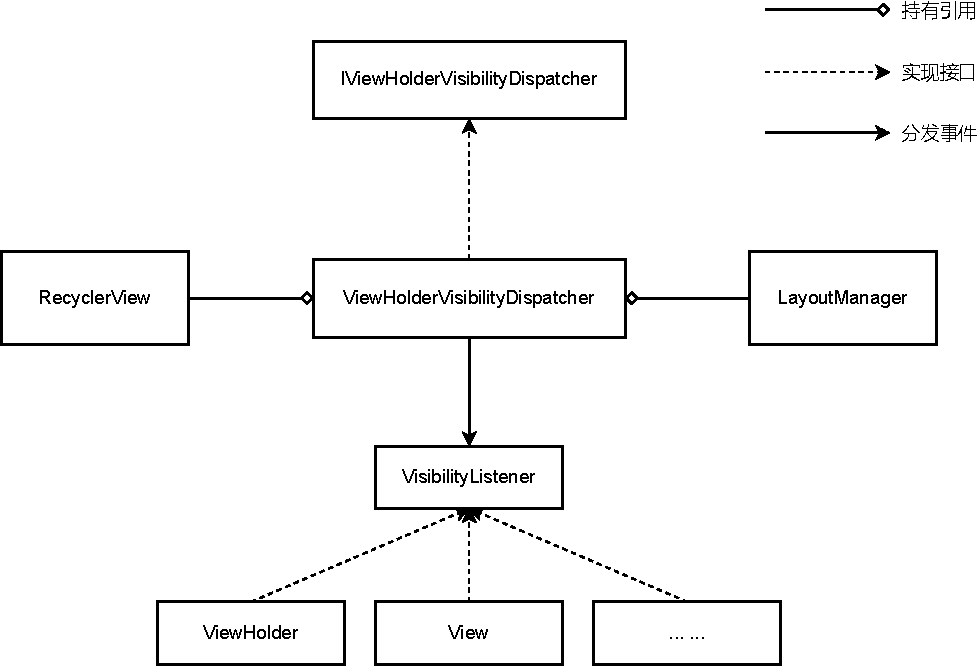
\includegraphics{assets/visibility-dispatch-framework.svg}}

\begin{figure}
    \centering
    \begin{adjustbox}{max width=\textwidth}
        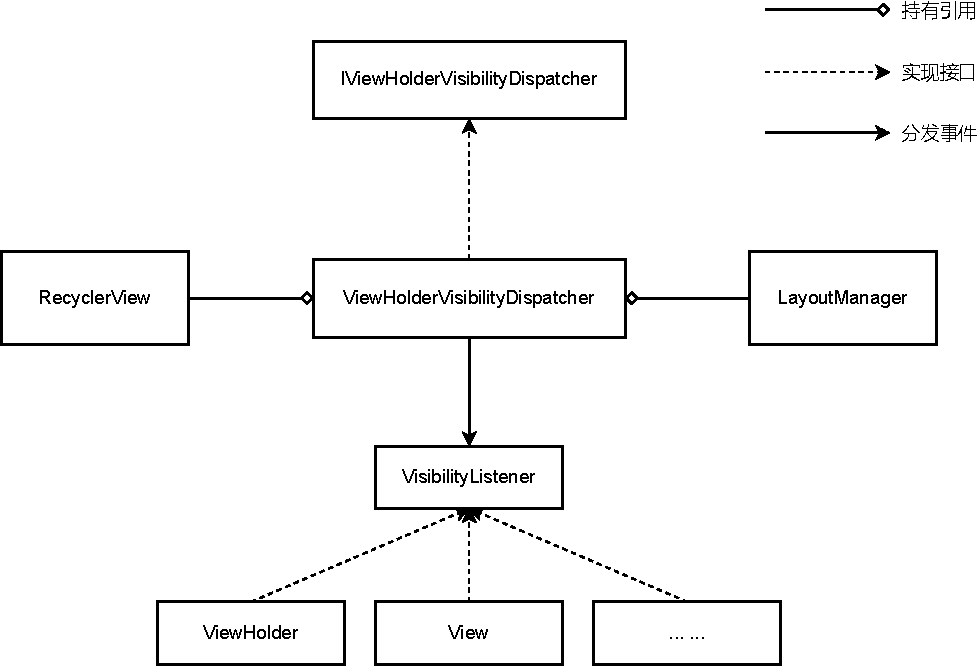
\includegraphics{assets/visibility-dispatch-framework.pdf}
    \end{adjustbox}
    \caption{可见性分发框架设计}
\end{figure}

% 可见性框架的细节

卡片可见性分发的框架设计如图 5.3。ViewHolderVisibilityDispatcher 是主要的卡片可见性事件分发组件,负责核心的可见性计算逻辑以及可见性的记忆和读取操作。由于 RecyclerView 和 LayoutManager 通常在业务中同时初始化,所以将绑定的逻辑也交给 ViewHolderVisibilityDispatcher,让其持有 RecyclerView 和 LayoutManager 的引用,来进行可见性的计算和分发。在相应的时机下,Dispatcher 会将对应的事件分发给 Listener,也就是卡片本身以及监听了可见性事件的业务方组件。在这样的设计模式下,业务方只需要将原来依赖于数据绑定的业务逻辑迁移到新的卡片可见性回调(也就是 VisibilityListener 中的方法)中即可。